\section{Appendix}\label{sec:appendix}

\setcounter{figure}{0}
\renewcommand{\thefigure}{S\arabic{figure}}
\renewcommand{\theHfigure}{S\arabic{figure}}

\subsection{GIAANN Development}\label{subsec:appendix-giaann-development}

\begin{figure}[p]
    \centering
    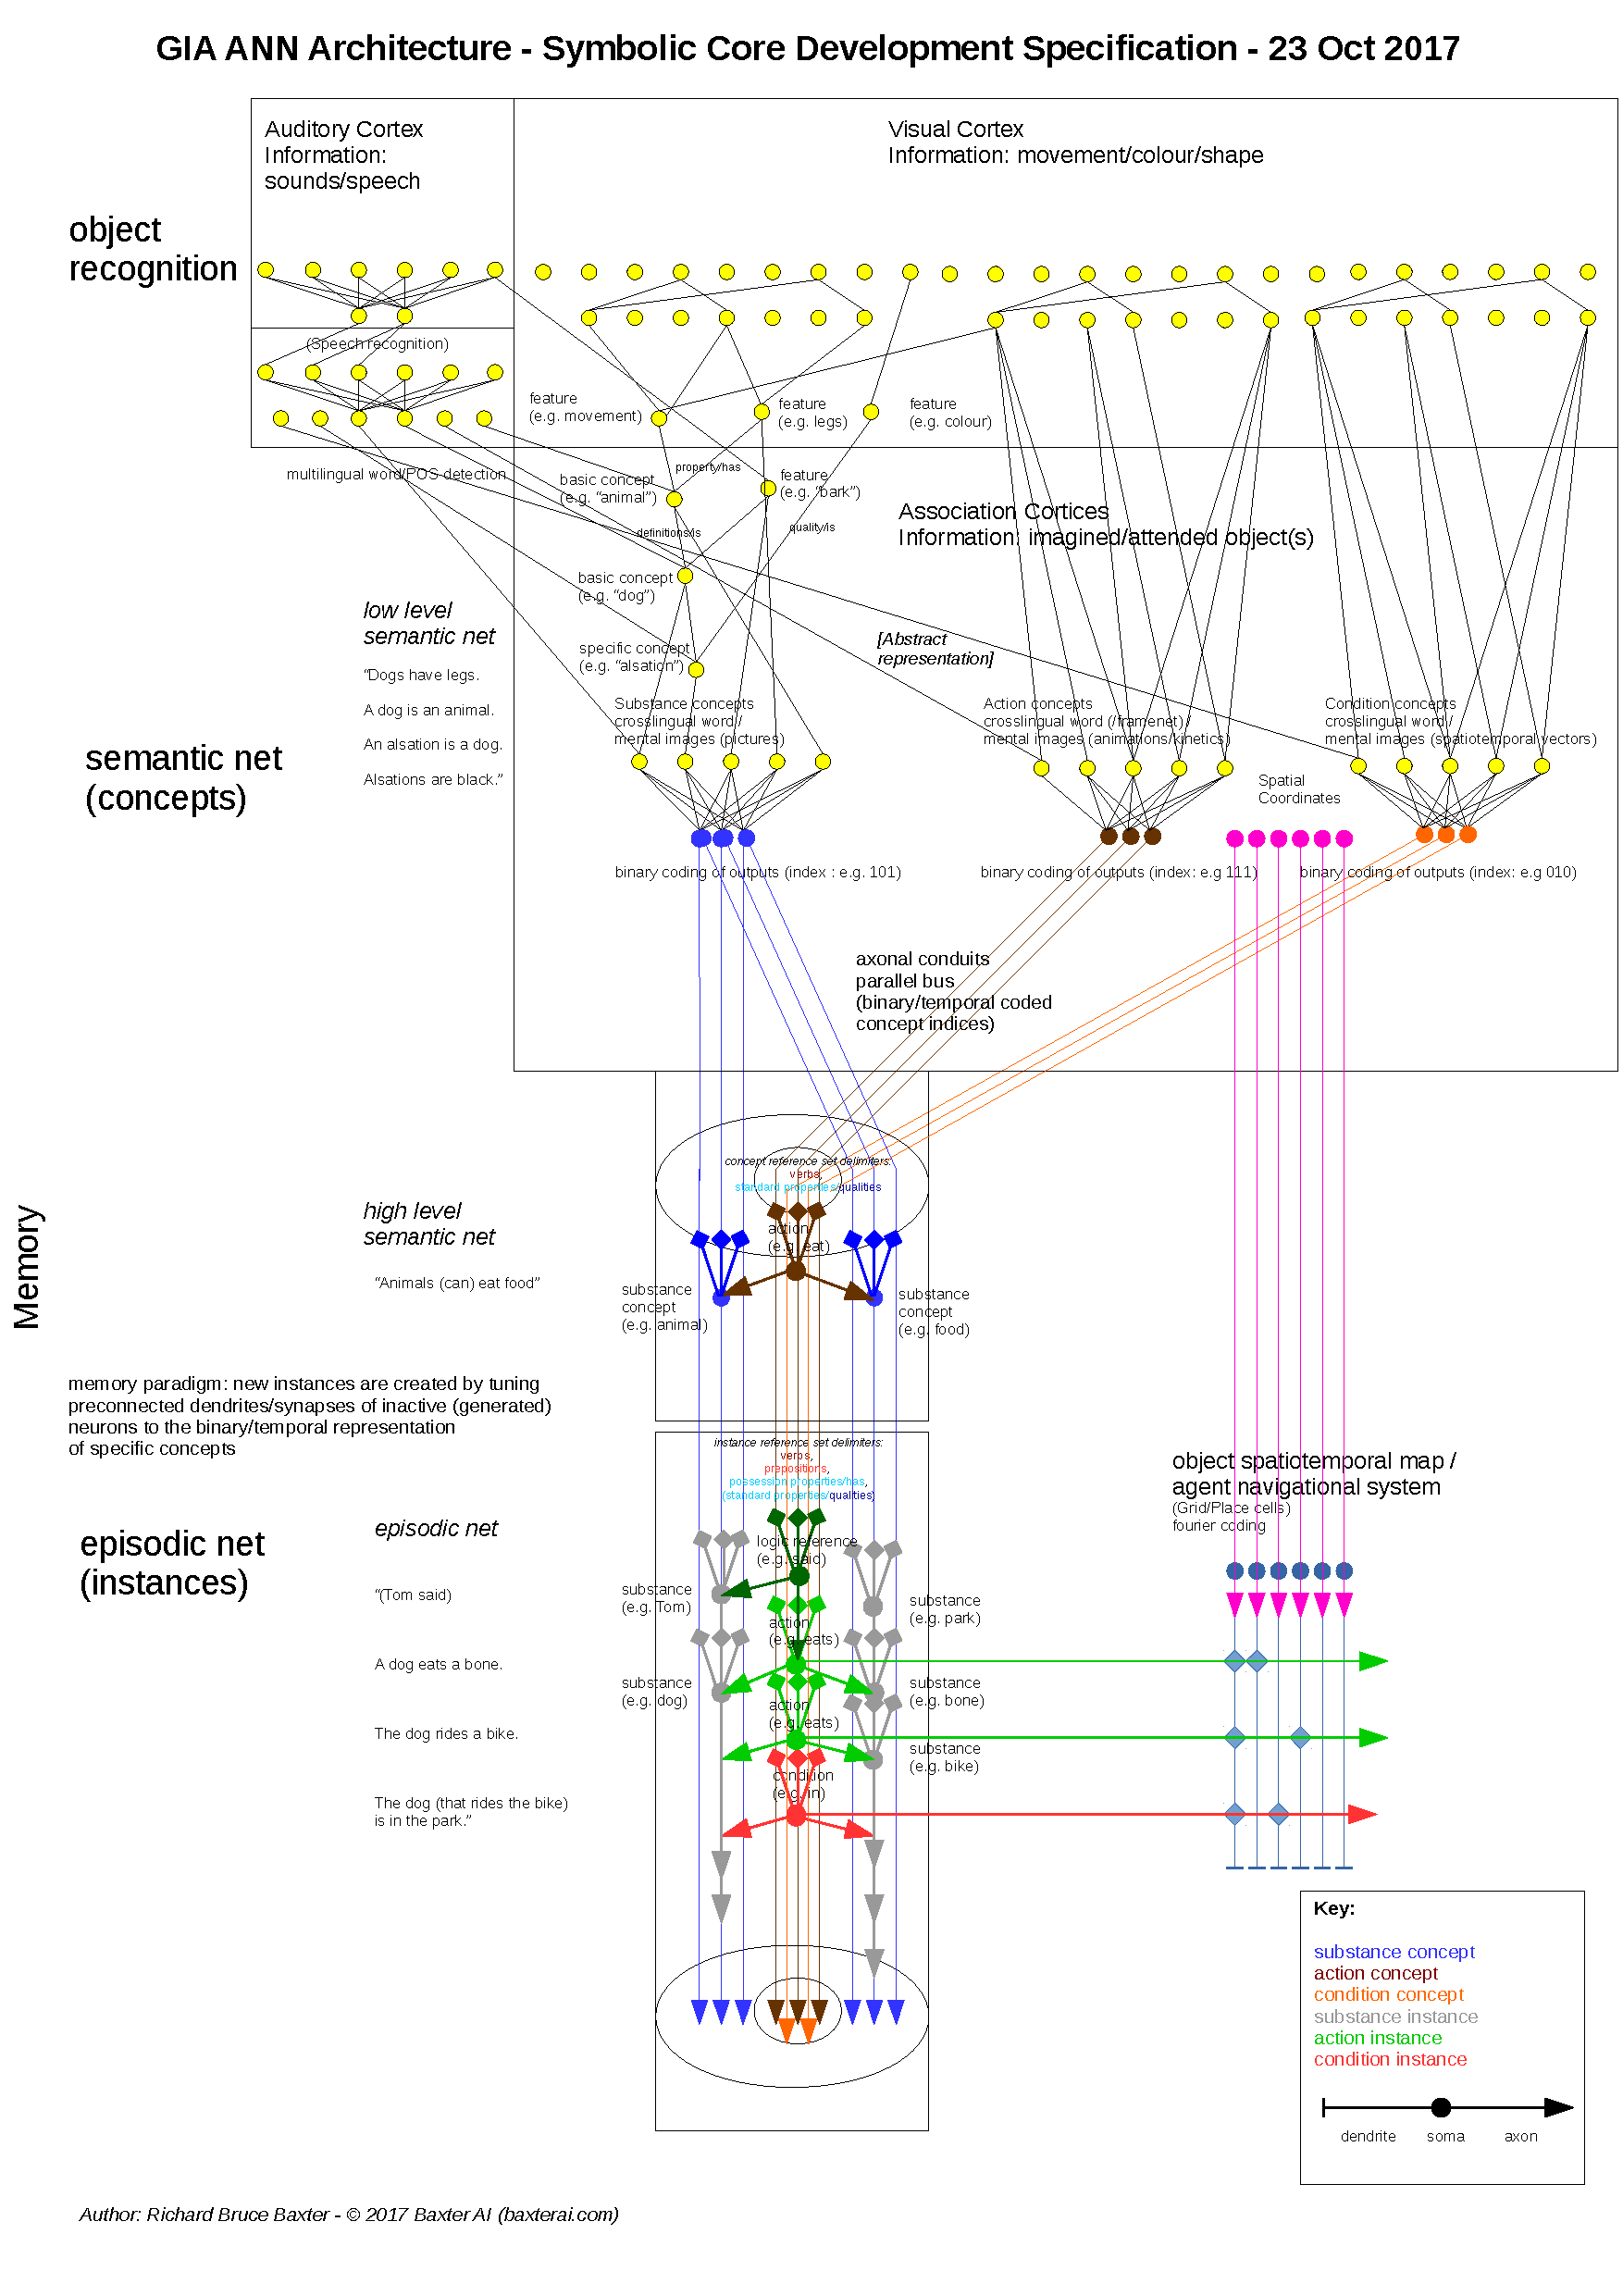
\includegraphics[width=\textwidth,height=0.88\textheight,keepaspectratio]{dev/GIAANNarchitectureDevelopment-23October2017a.pdf}
    \caption{Initial symbolic core with semantic concepts, episodic instances, and binary reference coding over axonal conduits.}
    \label{fig:dev-2017-initial-core}
\end{figure}
\clearpage

\begin{figure}[p]
    \centering
    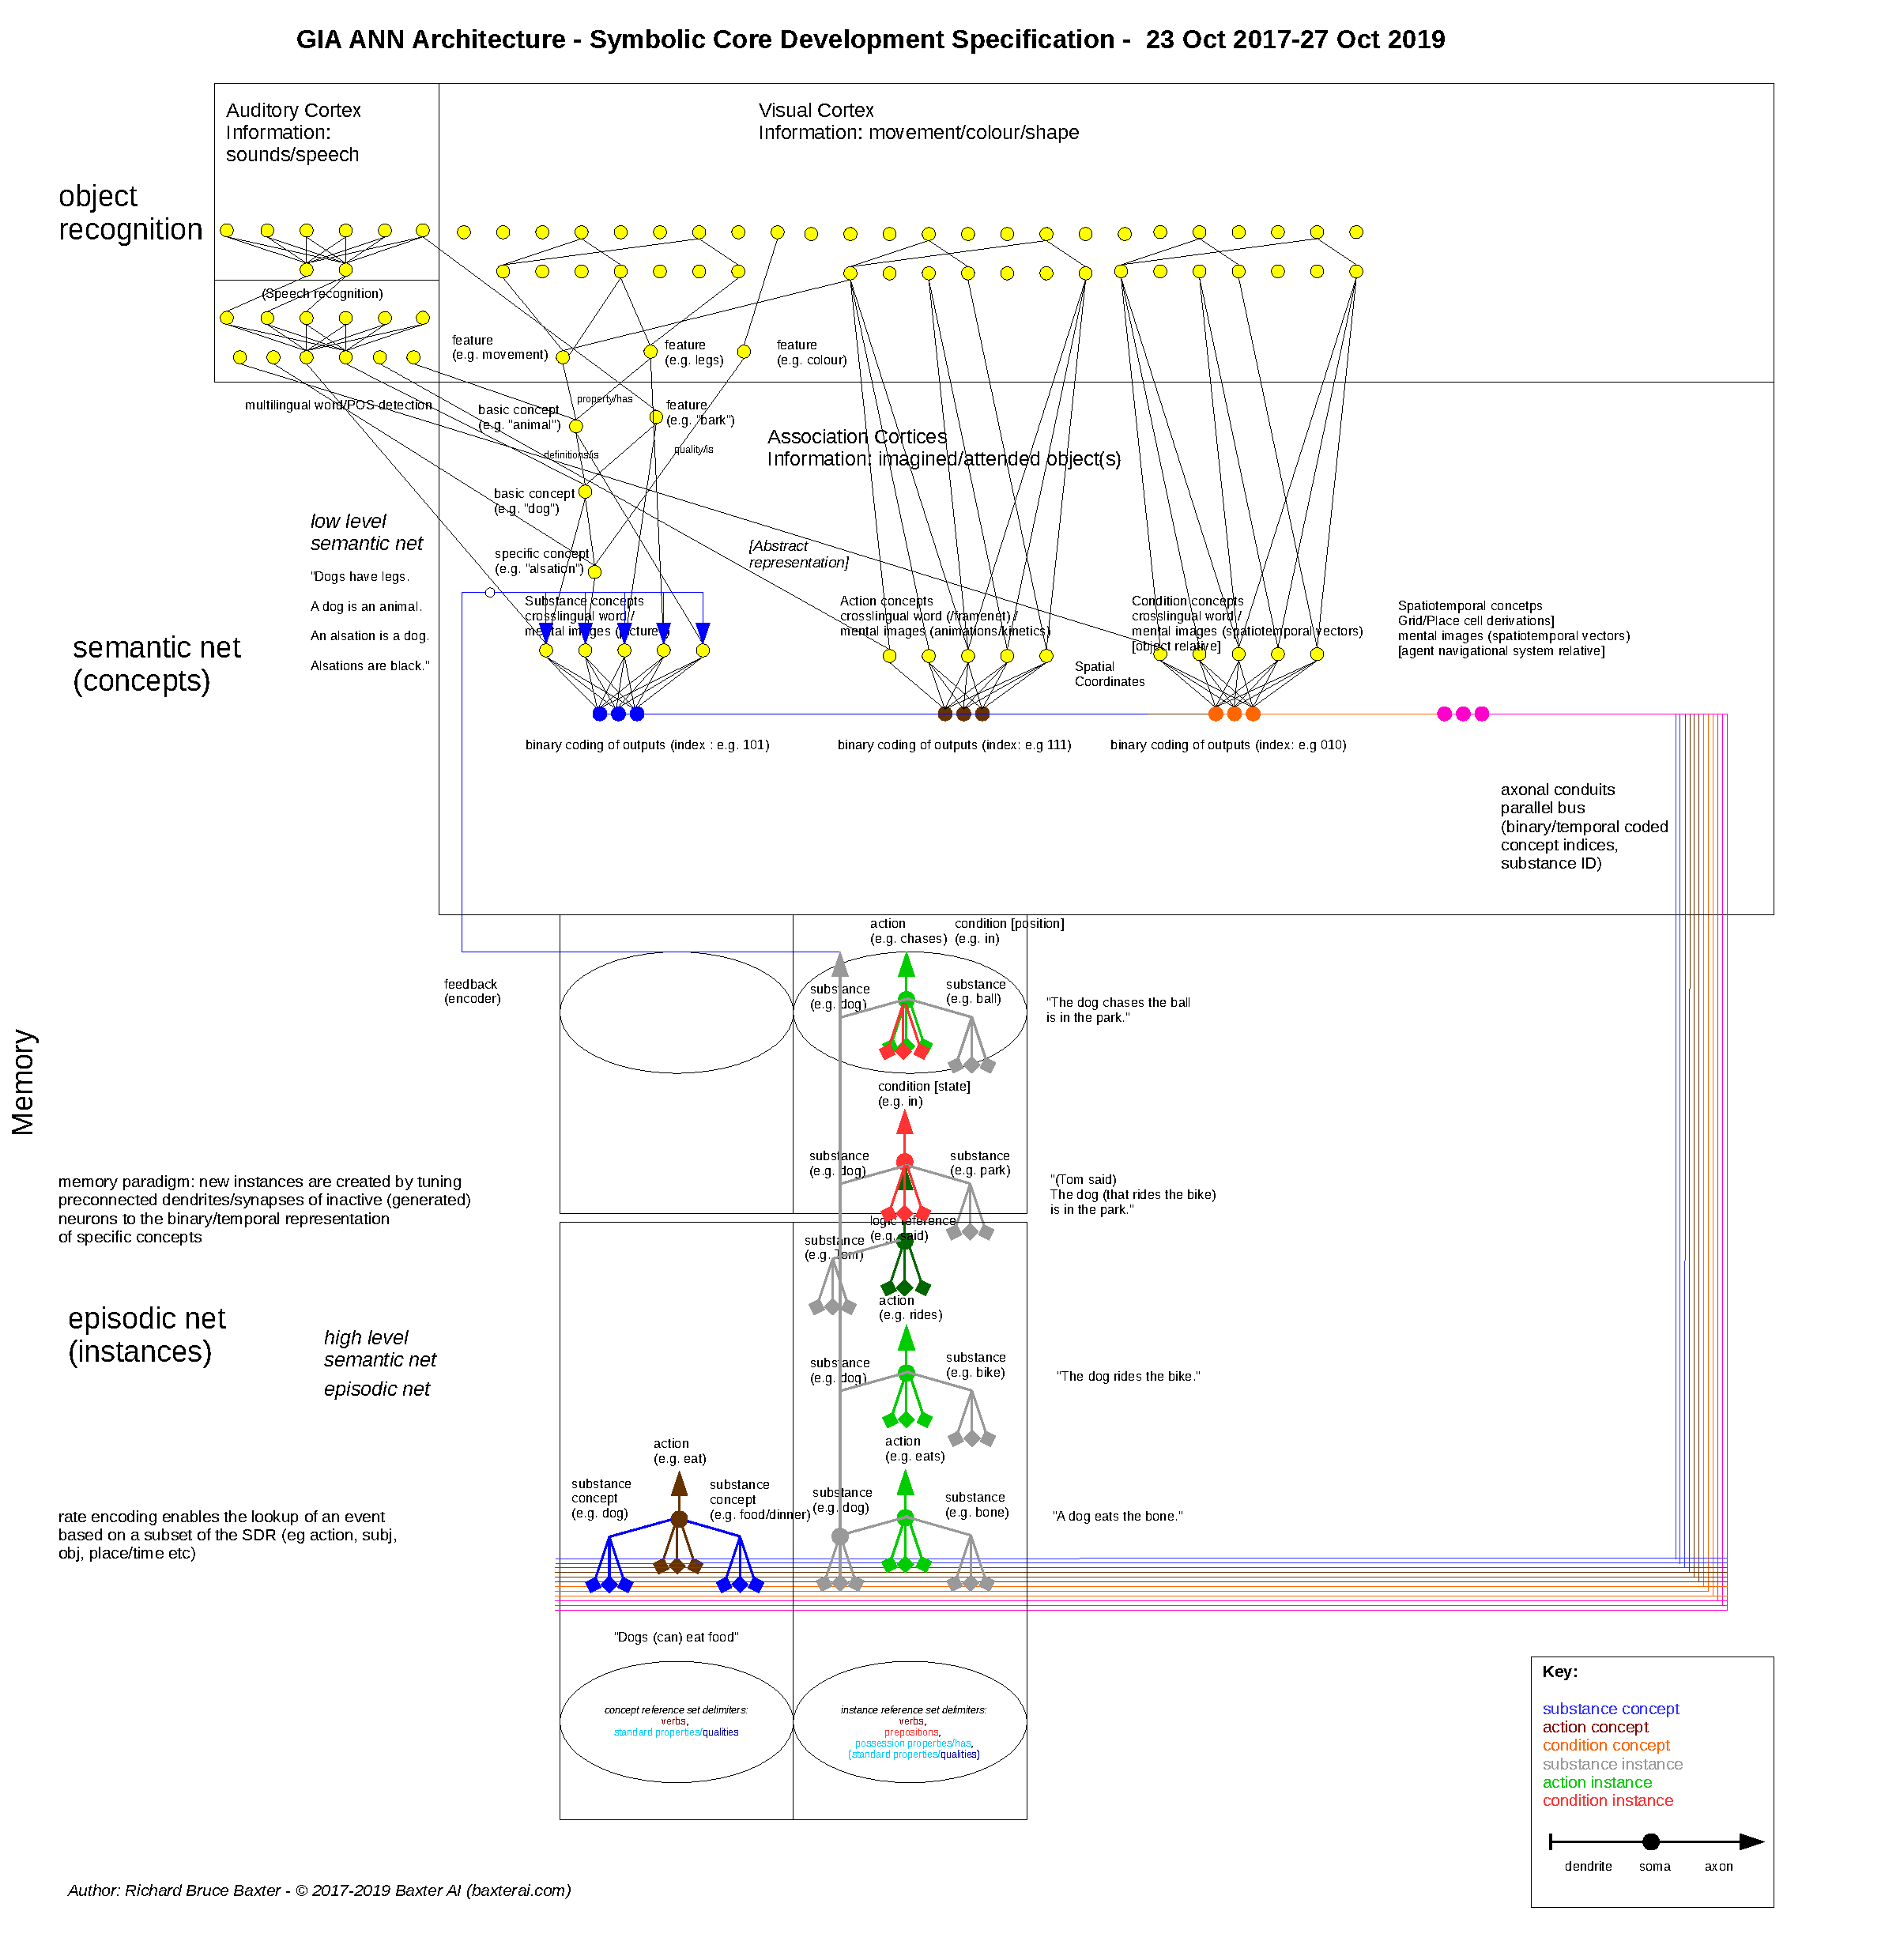
\includegraphics[width=\textwidth,height=0.88\textheight,keepaspectratio]{dev/GIAANNarchitectureDevelopment-27October2019a.pdf}
    \caption{Event retrieval refinement with feedback encoding and rate-coded lookup from partial cues (subject/action/object/place-time subsets).}
    \label{fig:dev-2019-event-retrieval}
\end{figure}
\clearpage

\begin{figure}[p]
    \centering
    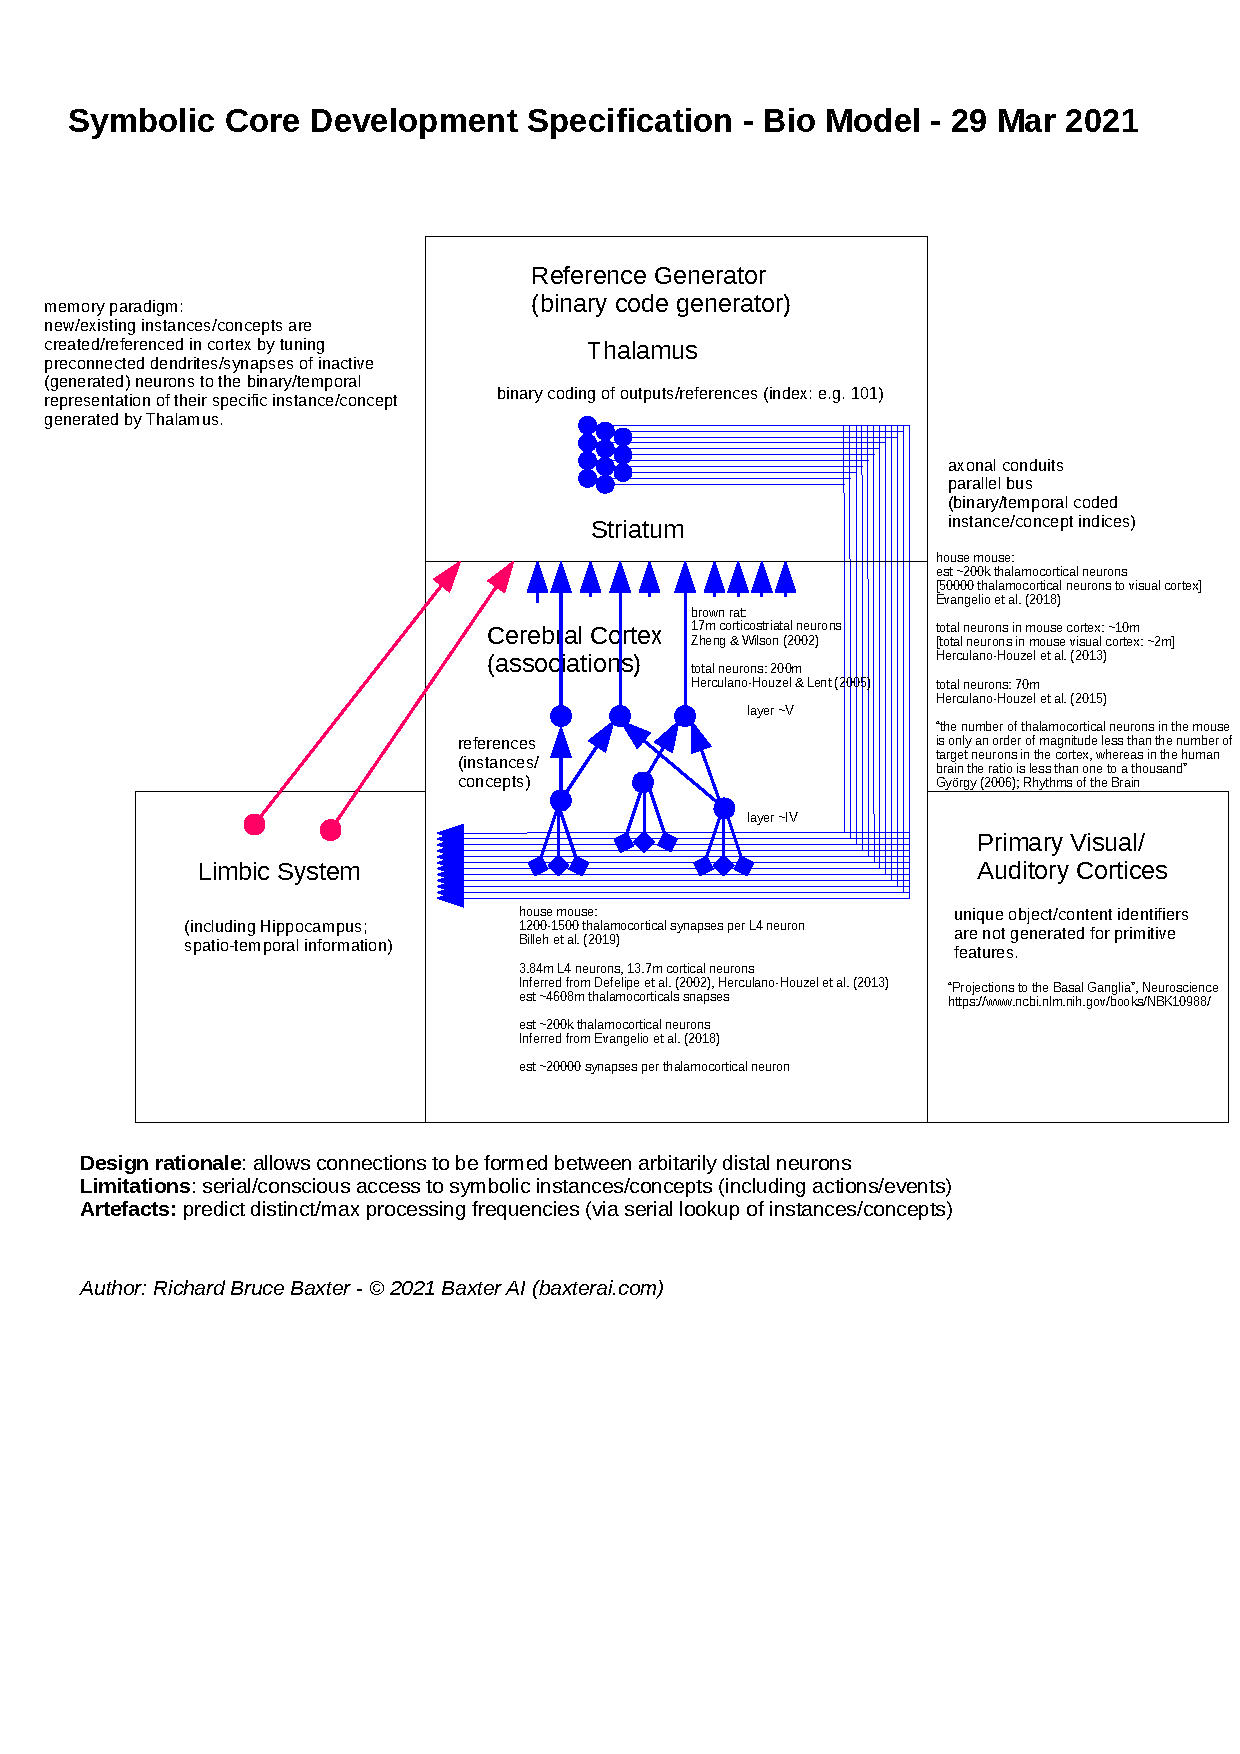
\includegraphics[width=\textwidth,height=0.88\textheight,keepaspectratio]{dev/GIAANNarchitectureDevelopment-bioModel-29March2021a.pdf}
    \caption{Bio-model mapping across thalamus, cortex, striatum, and limbic/hippocampal roles with design rationale and predicted serial-access constraints.}
    \label{fig:dev-2021-biomodel-mapping}
\end{figure}
\clearpage

\begin{figure}[p]
    \centering
    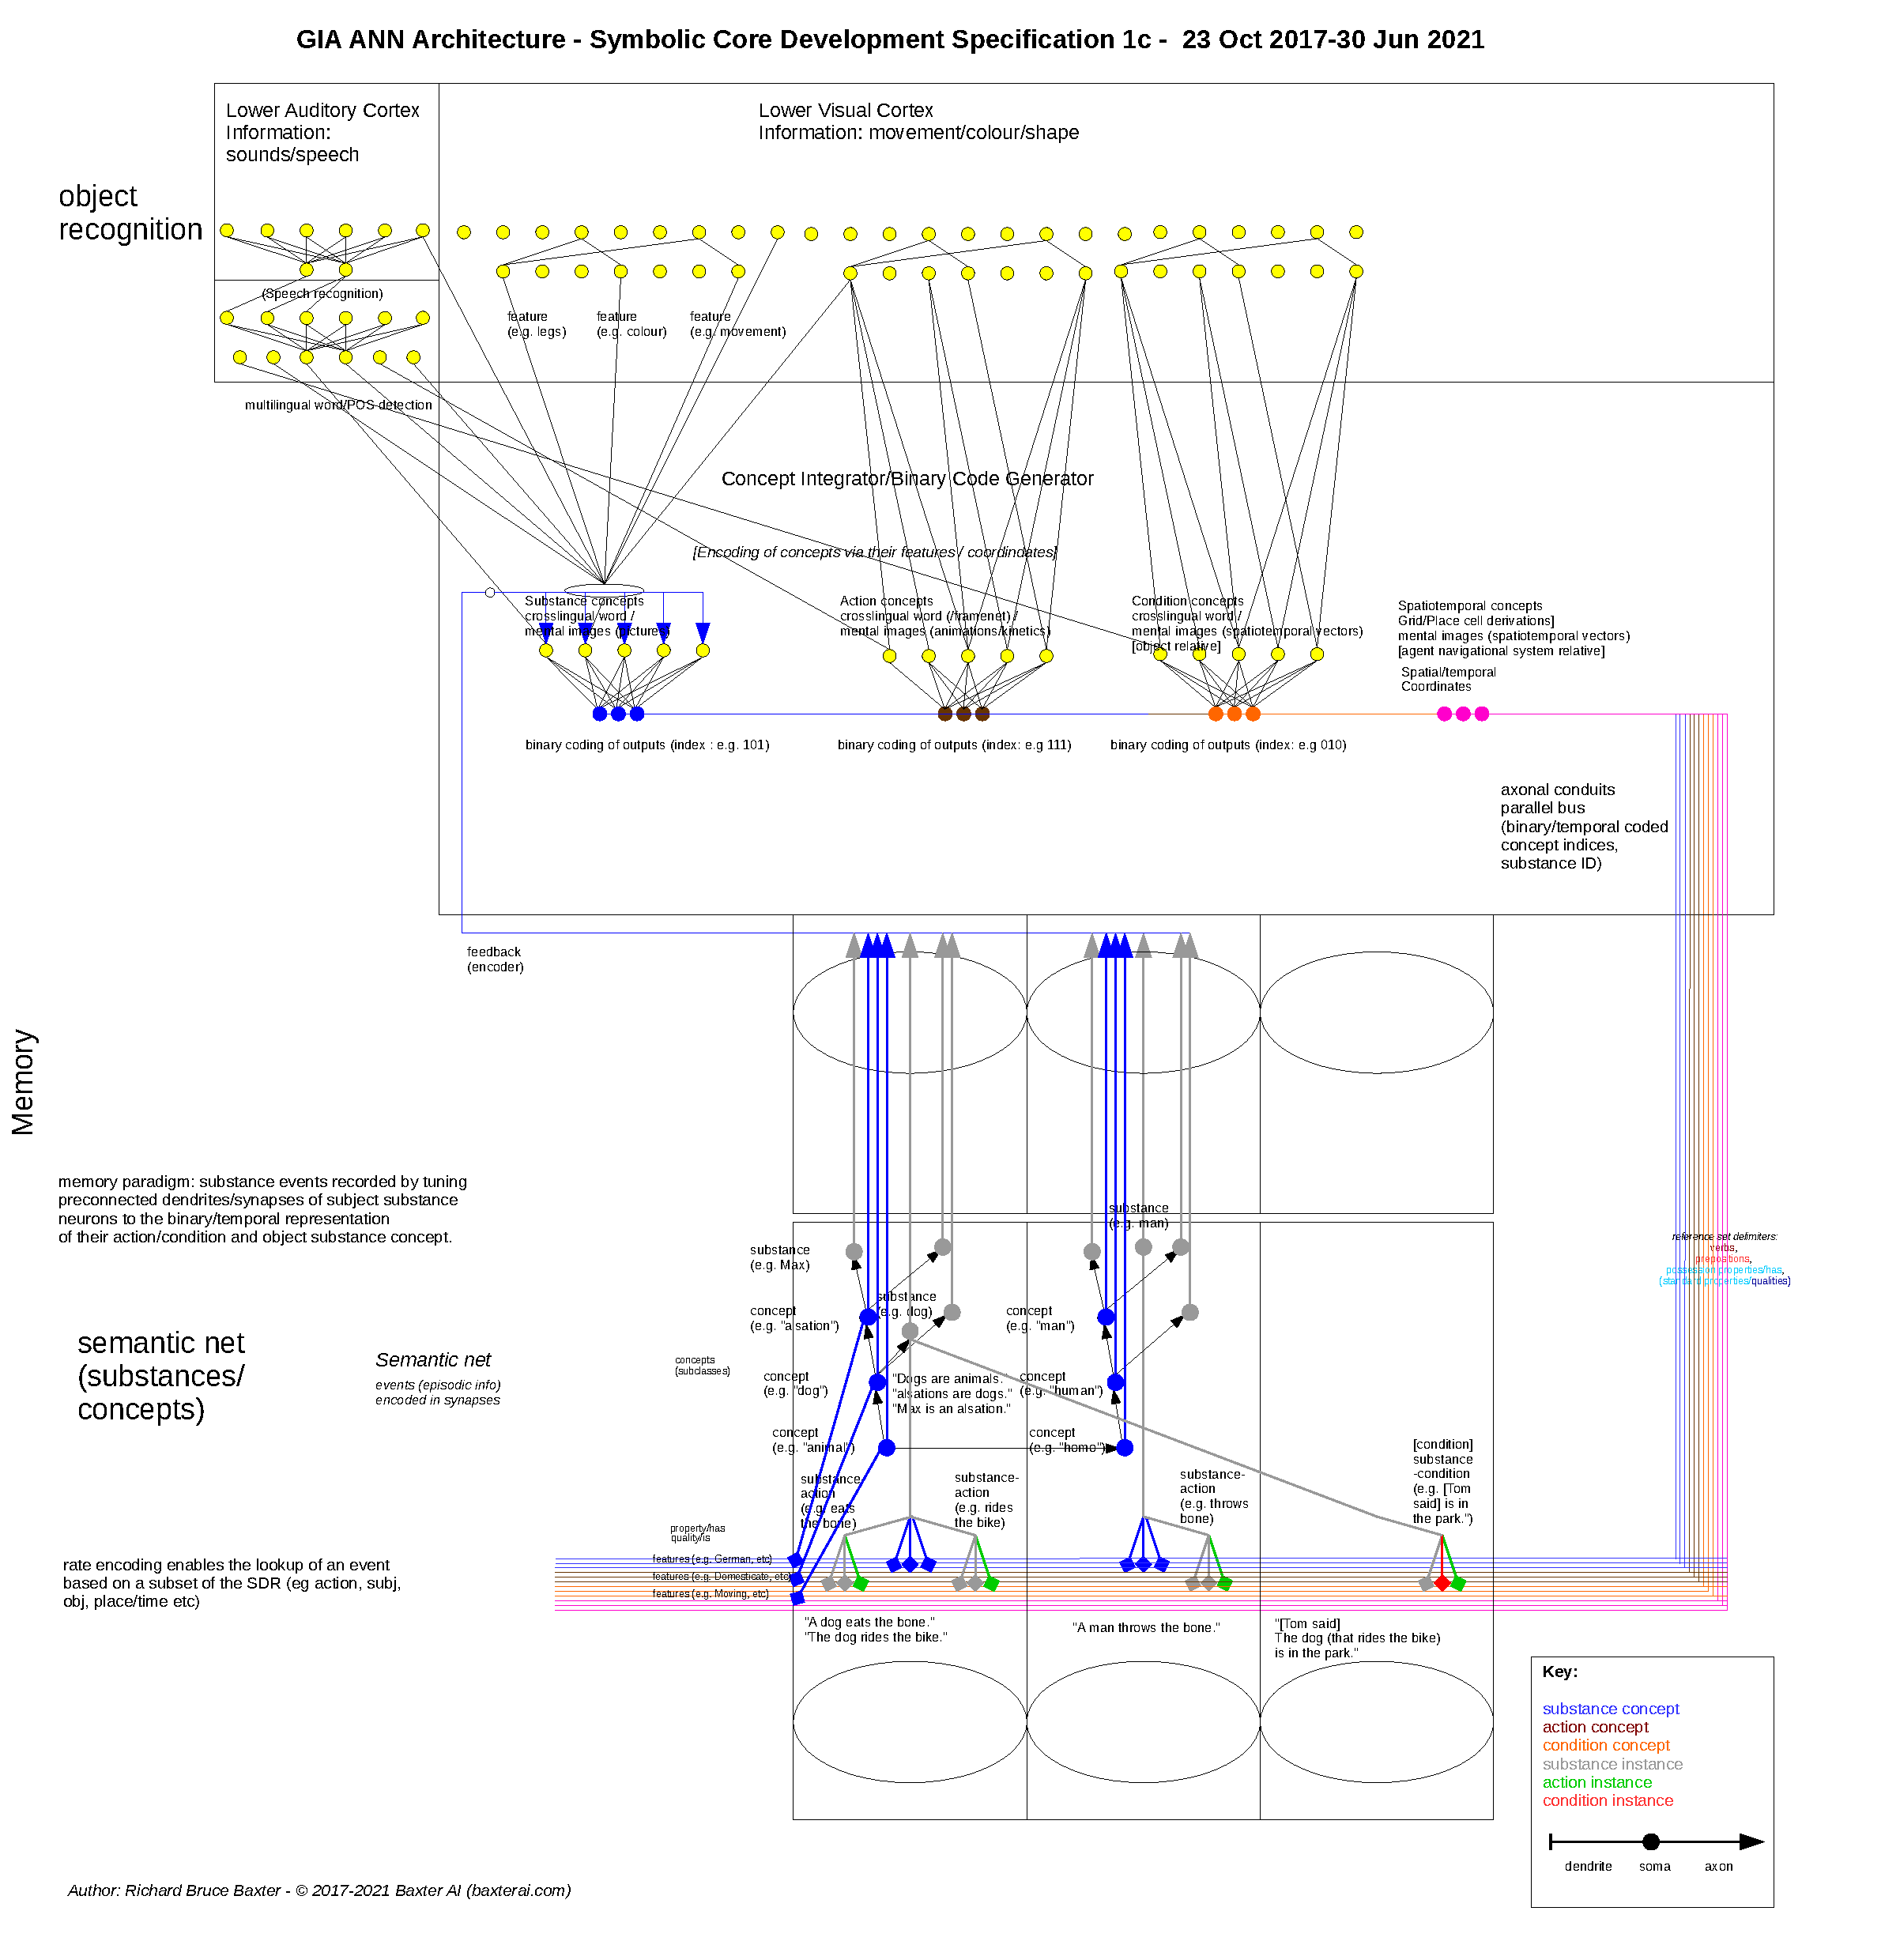
\includegraphics[width=\textwidth,height=0.88\textheight,keepaspectratio]{dev/GIAANNarchitectureDevelopment1c-30June2021a.pdf}
    \caption{Transition toward storing episodic information in synapses associated with substance/concept neurons, with a consolidated concept-integrator/reference-generator pathway.}
    \label{fig:dev-2021-synaptic-encoding}
\end{figure}
\clearpage

\begin{figure}[p]
    \centering
    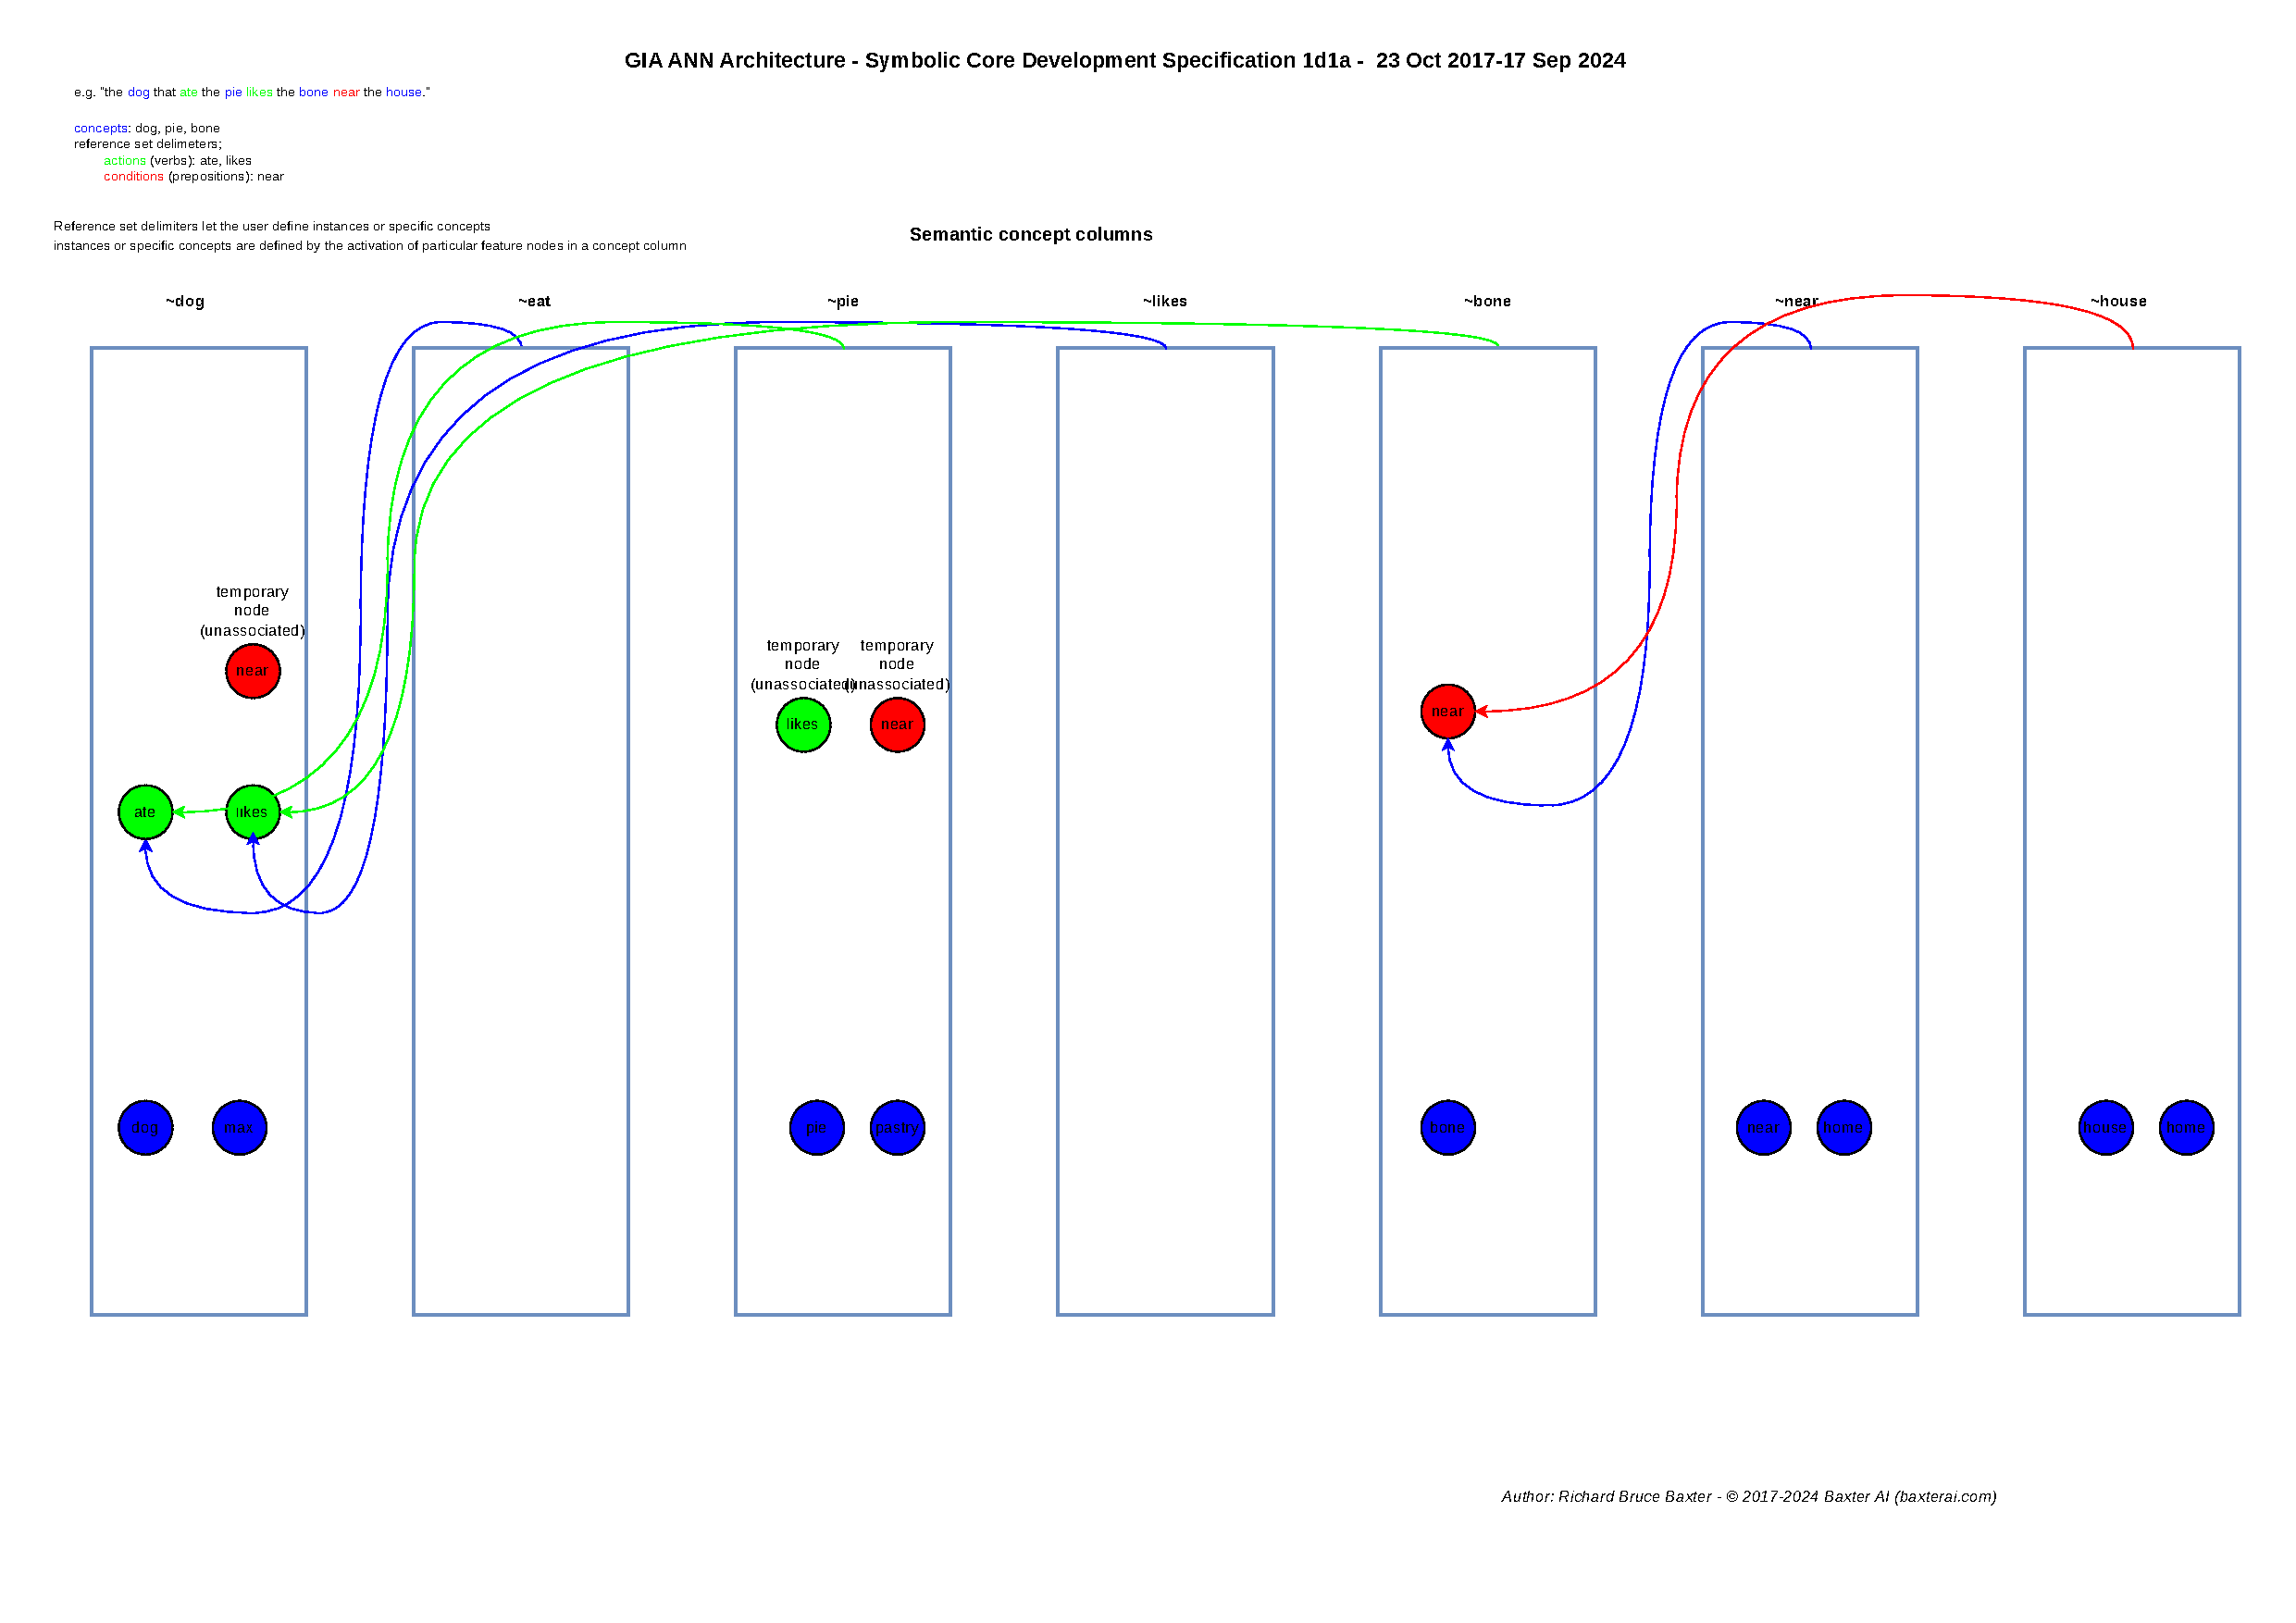
\includegraphics[width=\textwidth,height=0.88\textheight,keepaspectratio]{dev/GIAANNarchitectureDevelopment1d1a-17Sept2024a.pdf}
    \caption{Introduction of semantic concept columns and temporary unassociated nodes, with inter-column delimiter features (verbs and prepositions) used as routing constraints.}
    \label{fig:dev-2024-columns-routing}
\end{figure}
\clearpage

\begin{figure}[p]
    \centering
    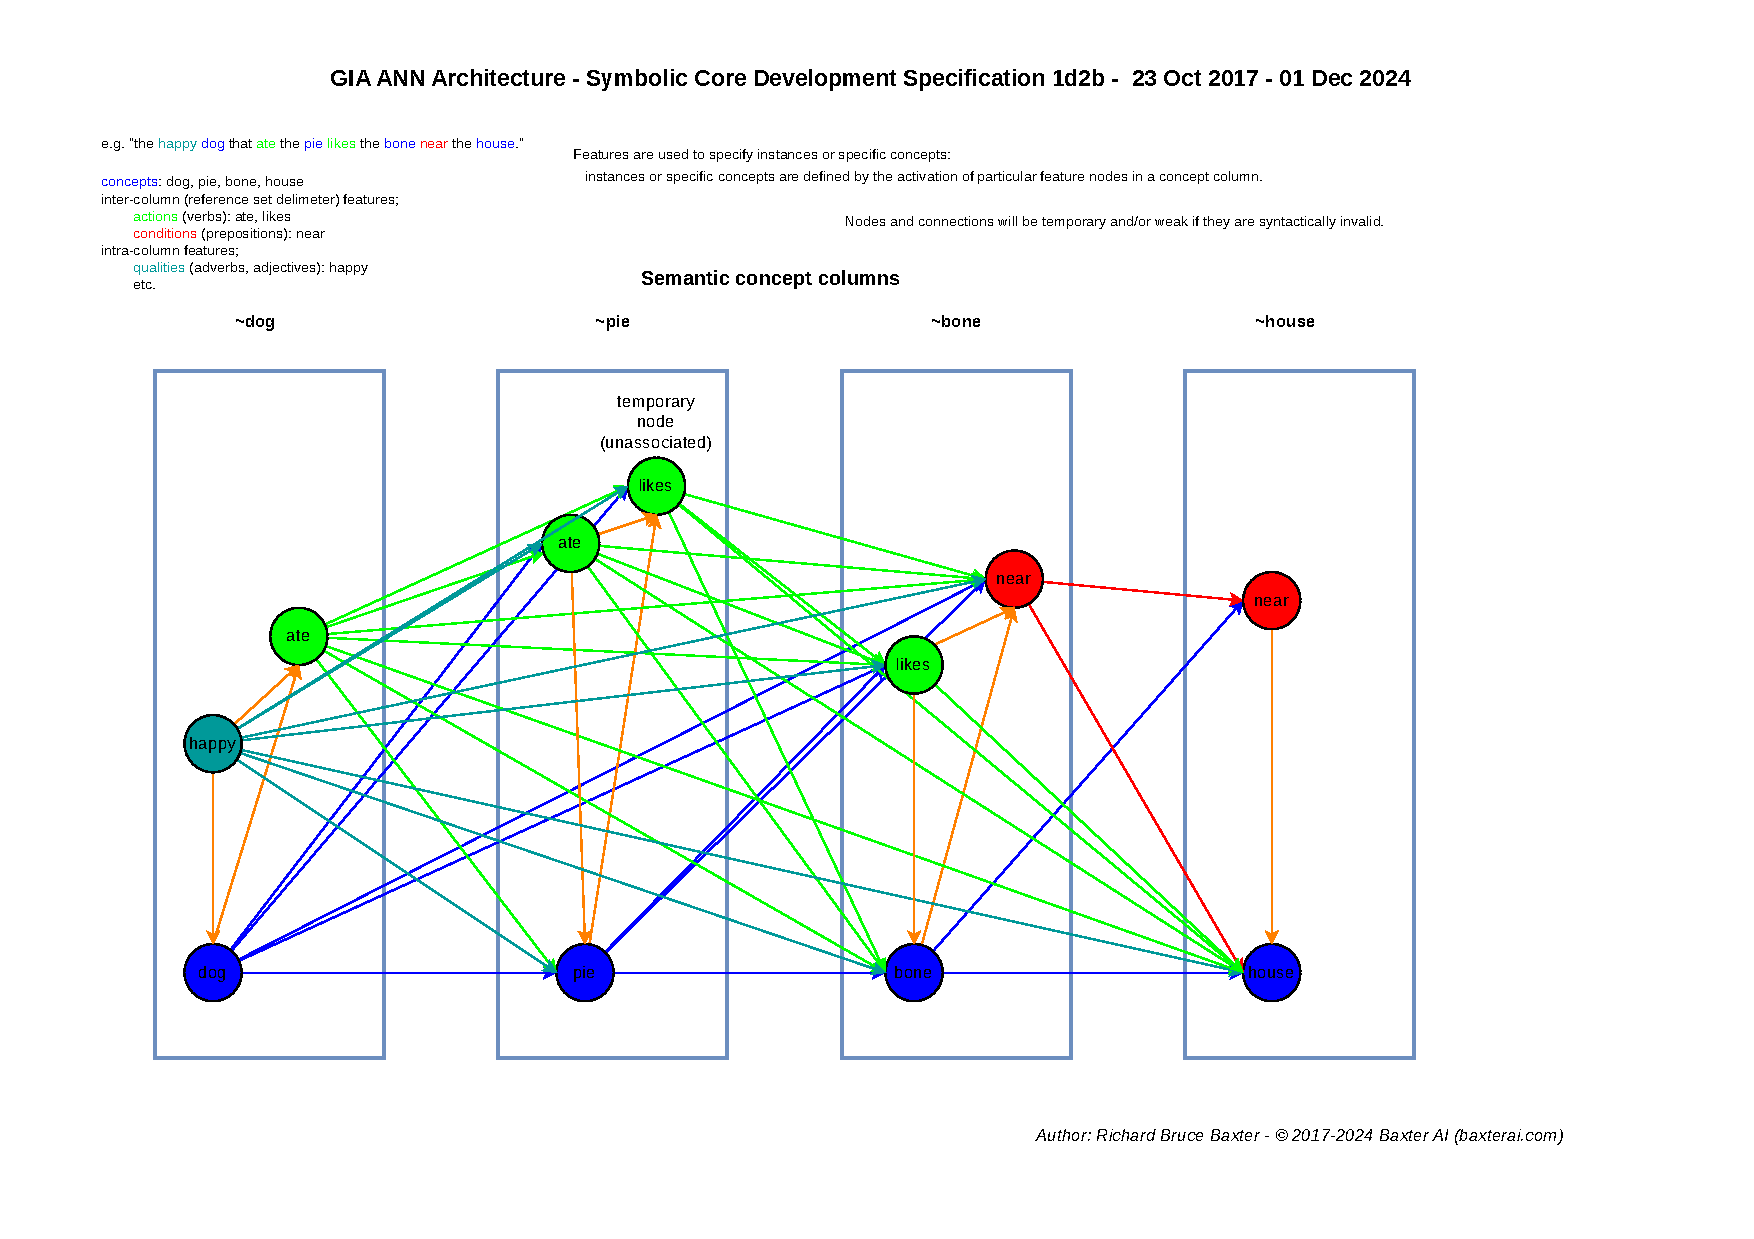
\includegraphics[width=\textwidth,height=0.88\textheight,keepaspectratio]{dev/GIAANNarchitectureDevelopment1d2b-01Dec2024a.pdf}
    \caption{Split between inter-column and intra-column features (e.g., qualities), plus syntactic-validity gating so invalid nodes/links remain weak or temporary.}
    \label{fig:dev-2024-feature-split-gating}
\end{figure}
\clearpage

\subsection{GIAANN Proto Specification}\label{subsec:appendix-giaann-proto-spec}

\noindent\textbf{File:} \texttt{dev/GIAANNproto1.nlc}

\lstinputlisting[
	language={},
	basicstyle=\scriptsize\rmfamily,
	breaklines=true,
	breakatwhitespace=true,
	columns=flexible,
	showstringspaces=false
]{dev/GIAANNproto1.nlc}